\section*{Zadanie 13.}
\begin{task}
Dany jest ośrodek o stałych $\mu,\ \epsilon,\ \sigma,$ w którym rozchodzi się płaska fala elektromagnetyczna. Narysować w skali podwójnie logarytmicznej wykresy współczynnika tłumienia oraz długości fali w funkcji częstotliwości. Jakie wnioski można stąd wyciągnąć odnośnie przesyłania fal radiowych w takich ośrodkach jak grunt czy woda morska? Zaznaczyć na wykresie obszar występowania efektu naskórkowego.\\
\end{task}

\begin{solution}


Zakładam, że dobry przewodnik, czyli: $\sigma=6*10^{7}\cfrac{S}{m}, \ \ \ \epsilon_{r}=\mu_{r}=1$.

\begin{center}
$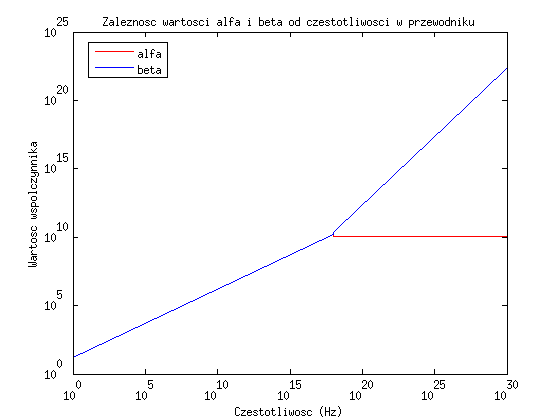
\includegraphics[scale=0.8]{13_1}$\\
\end{center}
\begin{center}
$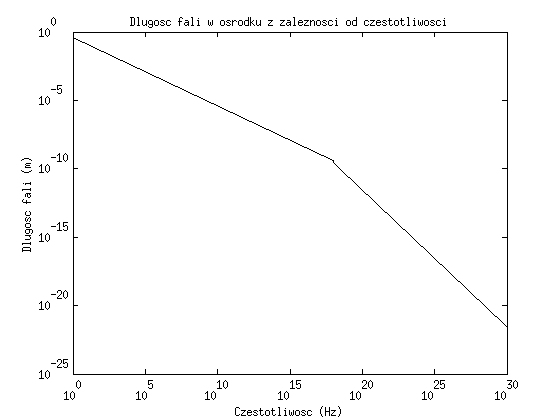
\includegraphics[scale=0.8]{13_2}$\\
\end{center}

Efekt naskórkowy występuje gdy $\alpha = \beta$, czyli w zakresie częstotliwości $10^{0} - 10^{18}$ Hz. Jednostki: $\alpha = \cfrac{1}{m}\ \ \ \beta=\cfrac{rad}{m}$.

\end{solution}